\appendices
\section{Additional Diagnostics}
\label{app:diagnostics}
\setlength{\textfloatsep}{8pt plus 2pt minus 2pt}
\setlength{\floatsep}{7pt plus 2pt minus 2pt}
\setlength{\intextsep}{7pt plus 2pt minus 2pt}
\setlength{\abovecaptionskip}{3pt}
\setlength{\belowcaptionskip}{2pt}

This appendix collects diagnostics that support the main results in
Table~\ref{tab:main_results}. Fig.~\ref{fig:queue_pressure} and
Fig.~\ref{fig:compact_policy_metrics} connect workload stress to the main
policy metrics. Figs.~\ref{fig:allocator_tradeoff}--\ref{fig:allocator_ablation_efficiency}
explain the Stage-2 allocator behavior behind Tables~\ref{tab:allocator_results}
and~\ref{tab:allocator_qos}. Table~\ref{tab:sla_thresholds}
lists the task-type SLA thresholds used for SLA and deadline-related QoS evaluation.

\subsection{Policy Stress and Metric Reading}

The edge queue response in Fig.~\ref{fig:queue_pressure} explains why the
offloading state includes queue-aware features. Bursty arrivals change the
local edge condition for multiple tasks at the same or nearby timesteps, so the
policy cannot rely only on task size or deadline.

\begin{figure}[H]
\centering
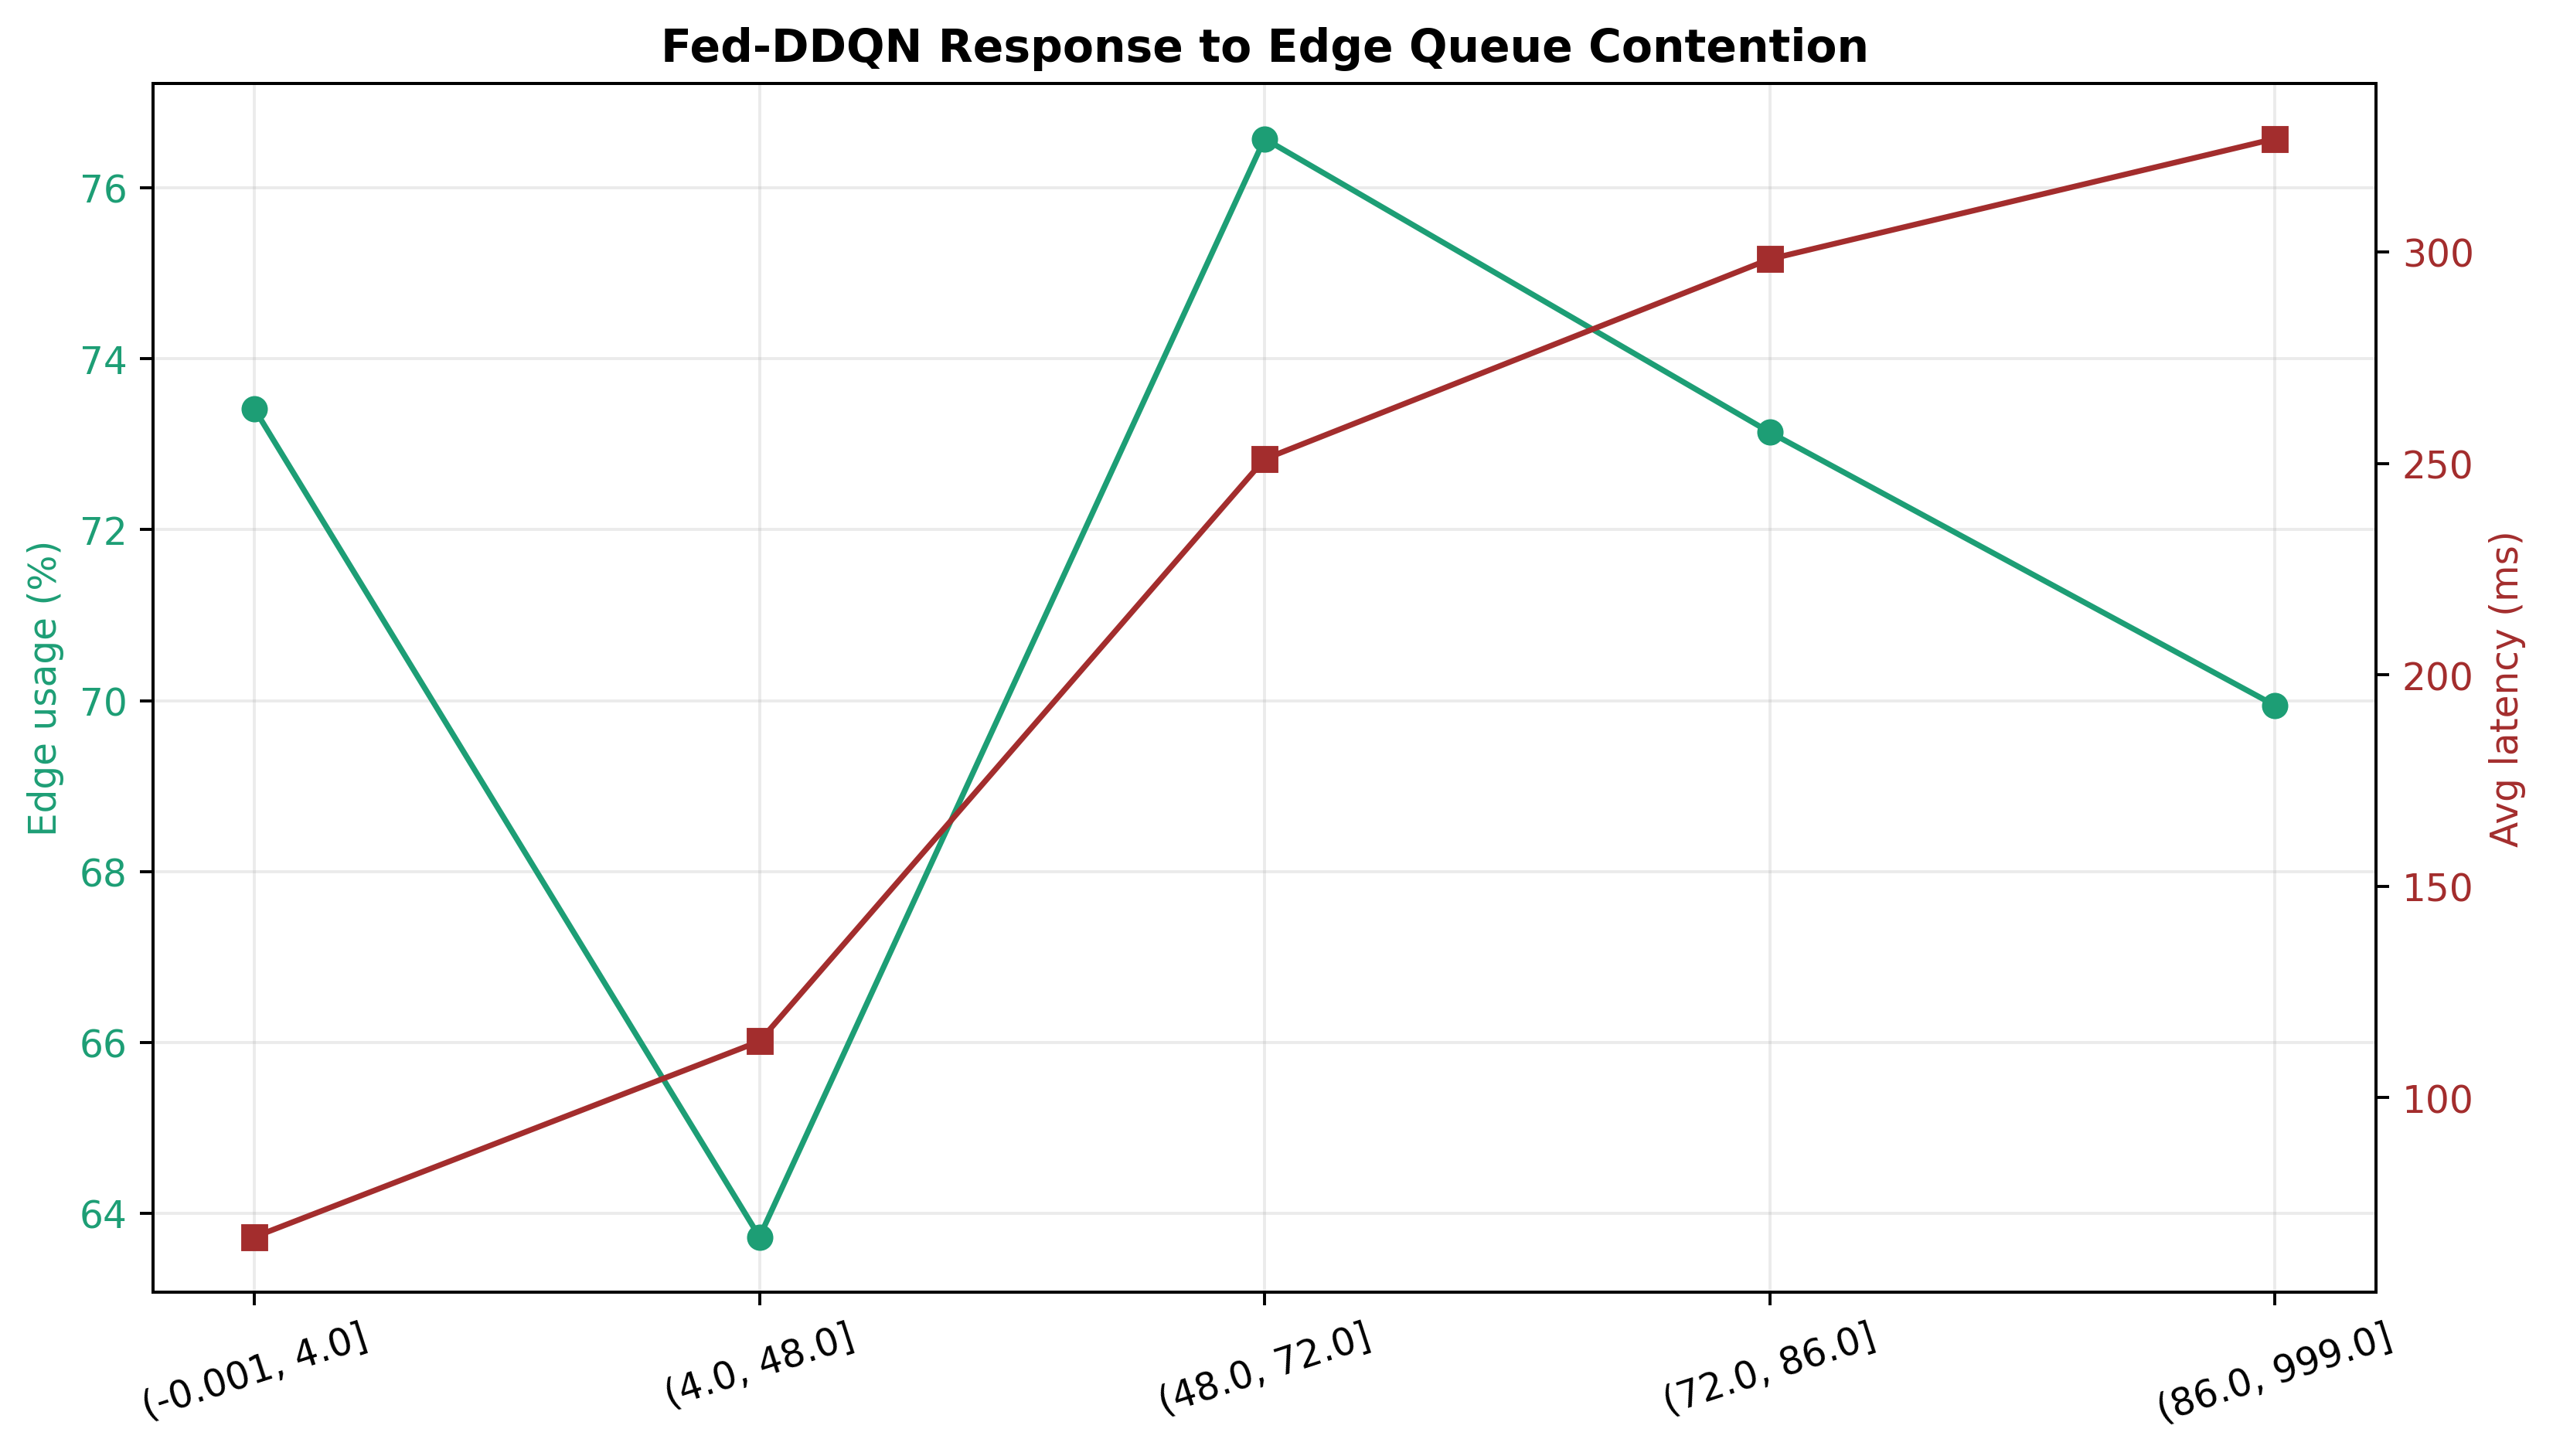
\includegraphics[width=0.82\columnwidth]{figures/diagnostics/165_fig_a18_edge_queue_pressure_response.png}
\caption{Edge queue pressure response under workload bursts.}
\label{fig:queue_pressure}
\end{figure}

The pattern to notice in Fig.~\ref{fig:queue_pressure} is the persistence of
queue pressure after a burst begins. It supports the use of temporal
train--validation--test splitting and queue-related state variables: a policy
trained only on independent task samples would not observe the same delayed
effect of contention on nearby tasks. It also explains why edge selection must
be moderated during burst windows even when individual tasks look edge
favorable in isolation.

\begin{figure}[H]
\centering
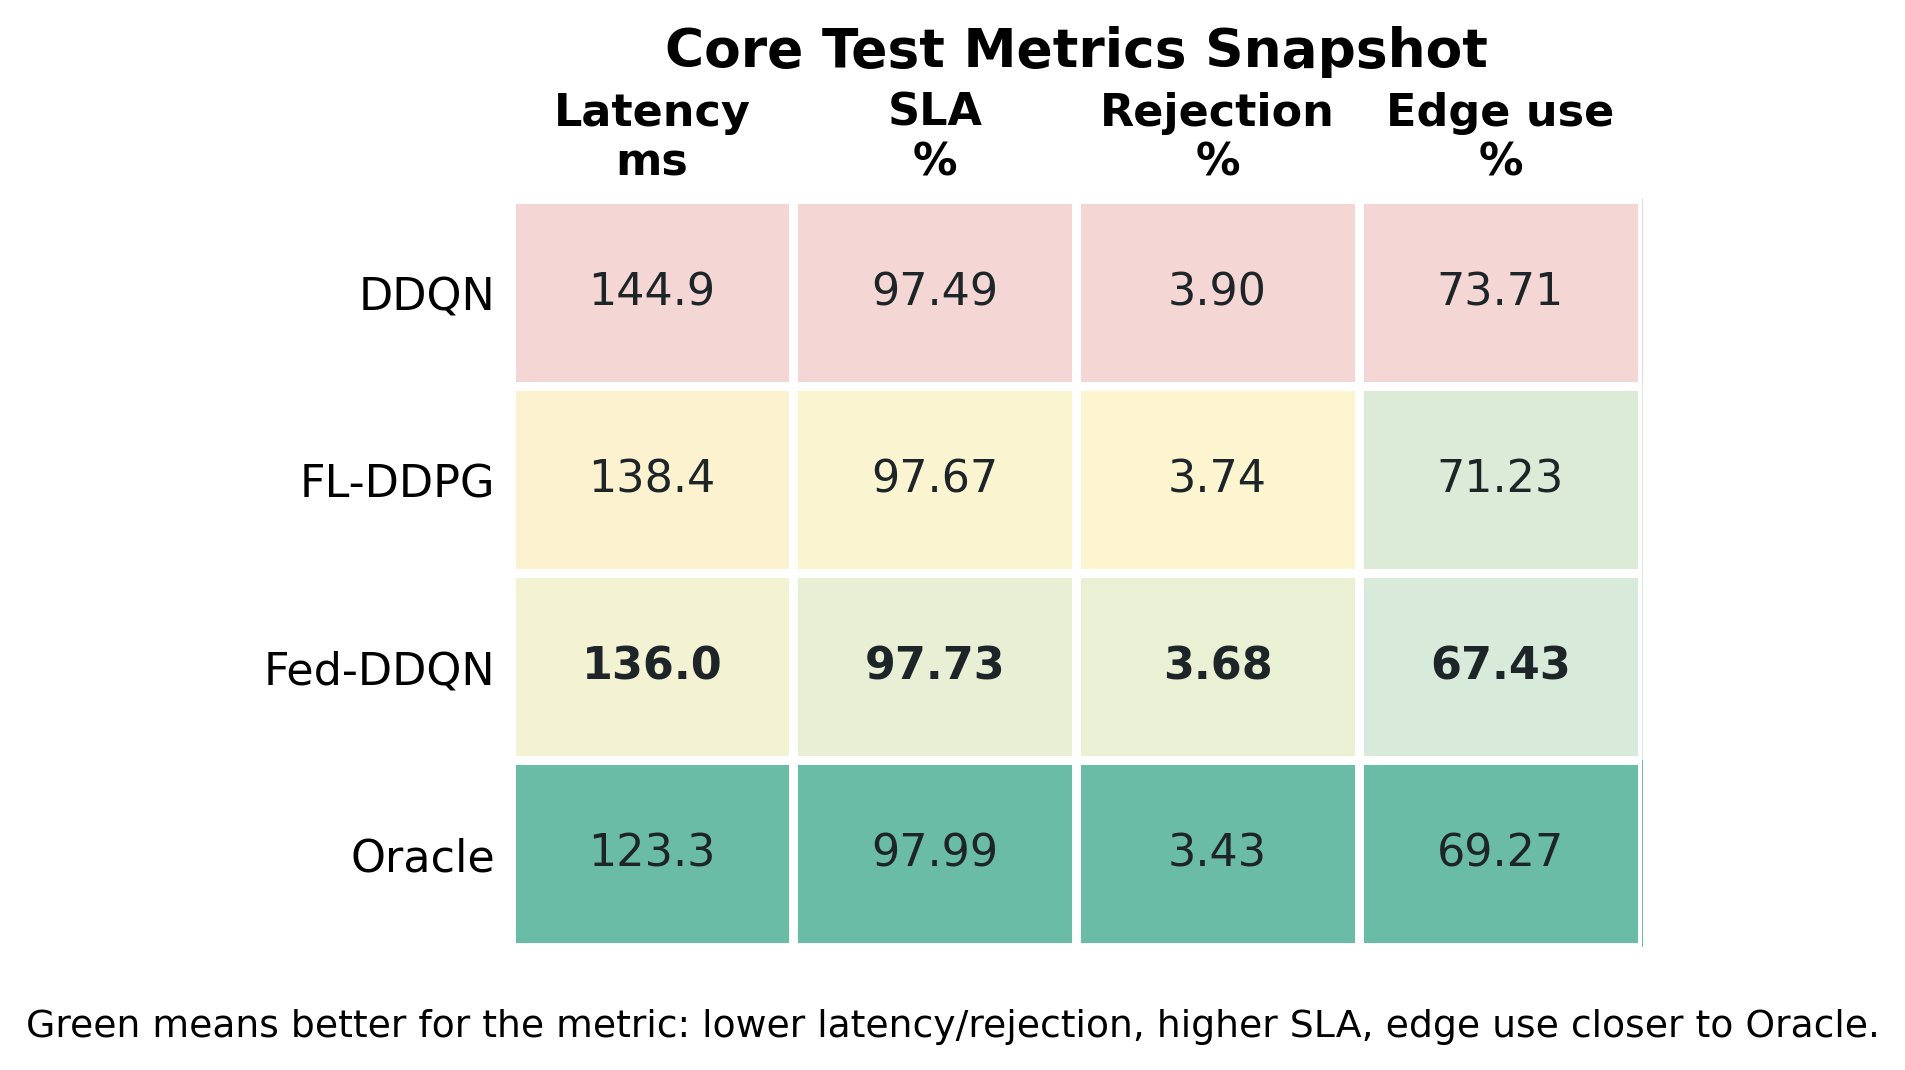
\includegraphics[width=0.94\columnwidth]{figures/diagnostics/173_fig_a26_policy_metric_snapshot.png}
\caption{Core test-metric snapshot for the closest trainable comparators and the latency-reference Oracle. Green cells indicate the preferred direction for each metric: lower latency and rejection, higher SLA, and edge usage closer to Oracle.}
\label{fig:compact_policy_metrics}
\end{figure}

The metric snapshot in Fig.~\ref{fig:compact_policy_metrics} gives a direct
reader-facing summary of the main policy tradeoff. It keeps the proposed model
beside DDQN, FL-DDPG, and Oracle, so the latency gain can be read together with
SLA, rejection, and destination balance. Stage 1 is judged by these policy
metrics, while Stage 2 is judged separately by allocation error,
under-allocation, waste, capacity violation, and risk-aware efficiency. The two
views should not be collapsed into one number.

\subsection{Stage-2 Allocator Diagnostics}

The allocator diagnostics separate error, feasibility, and QoS behavior. A
method with low mean error can still be poor if it violates capacity or
under-allocates deadline-sensitive tasks. Fig.~\ref{fig:allocator_tradeoff}
summarizes the tradeoff across all allocator variants. Fig.~\ref{fig:allocator_profile}
shows the under-allocation and excess profile after capacity normalization.
Fig.~\ref{fig:allocator_target_distribution} compares target and assigned
resource distributions, while Fig.~\ref{fig:stage2_task_mix} shows which task
types enter Stage 2 after the proposed offloading policy selects edge
execution.

\begin{figure}[H]
\centering
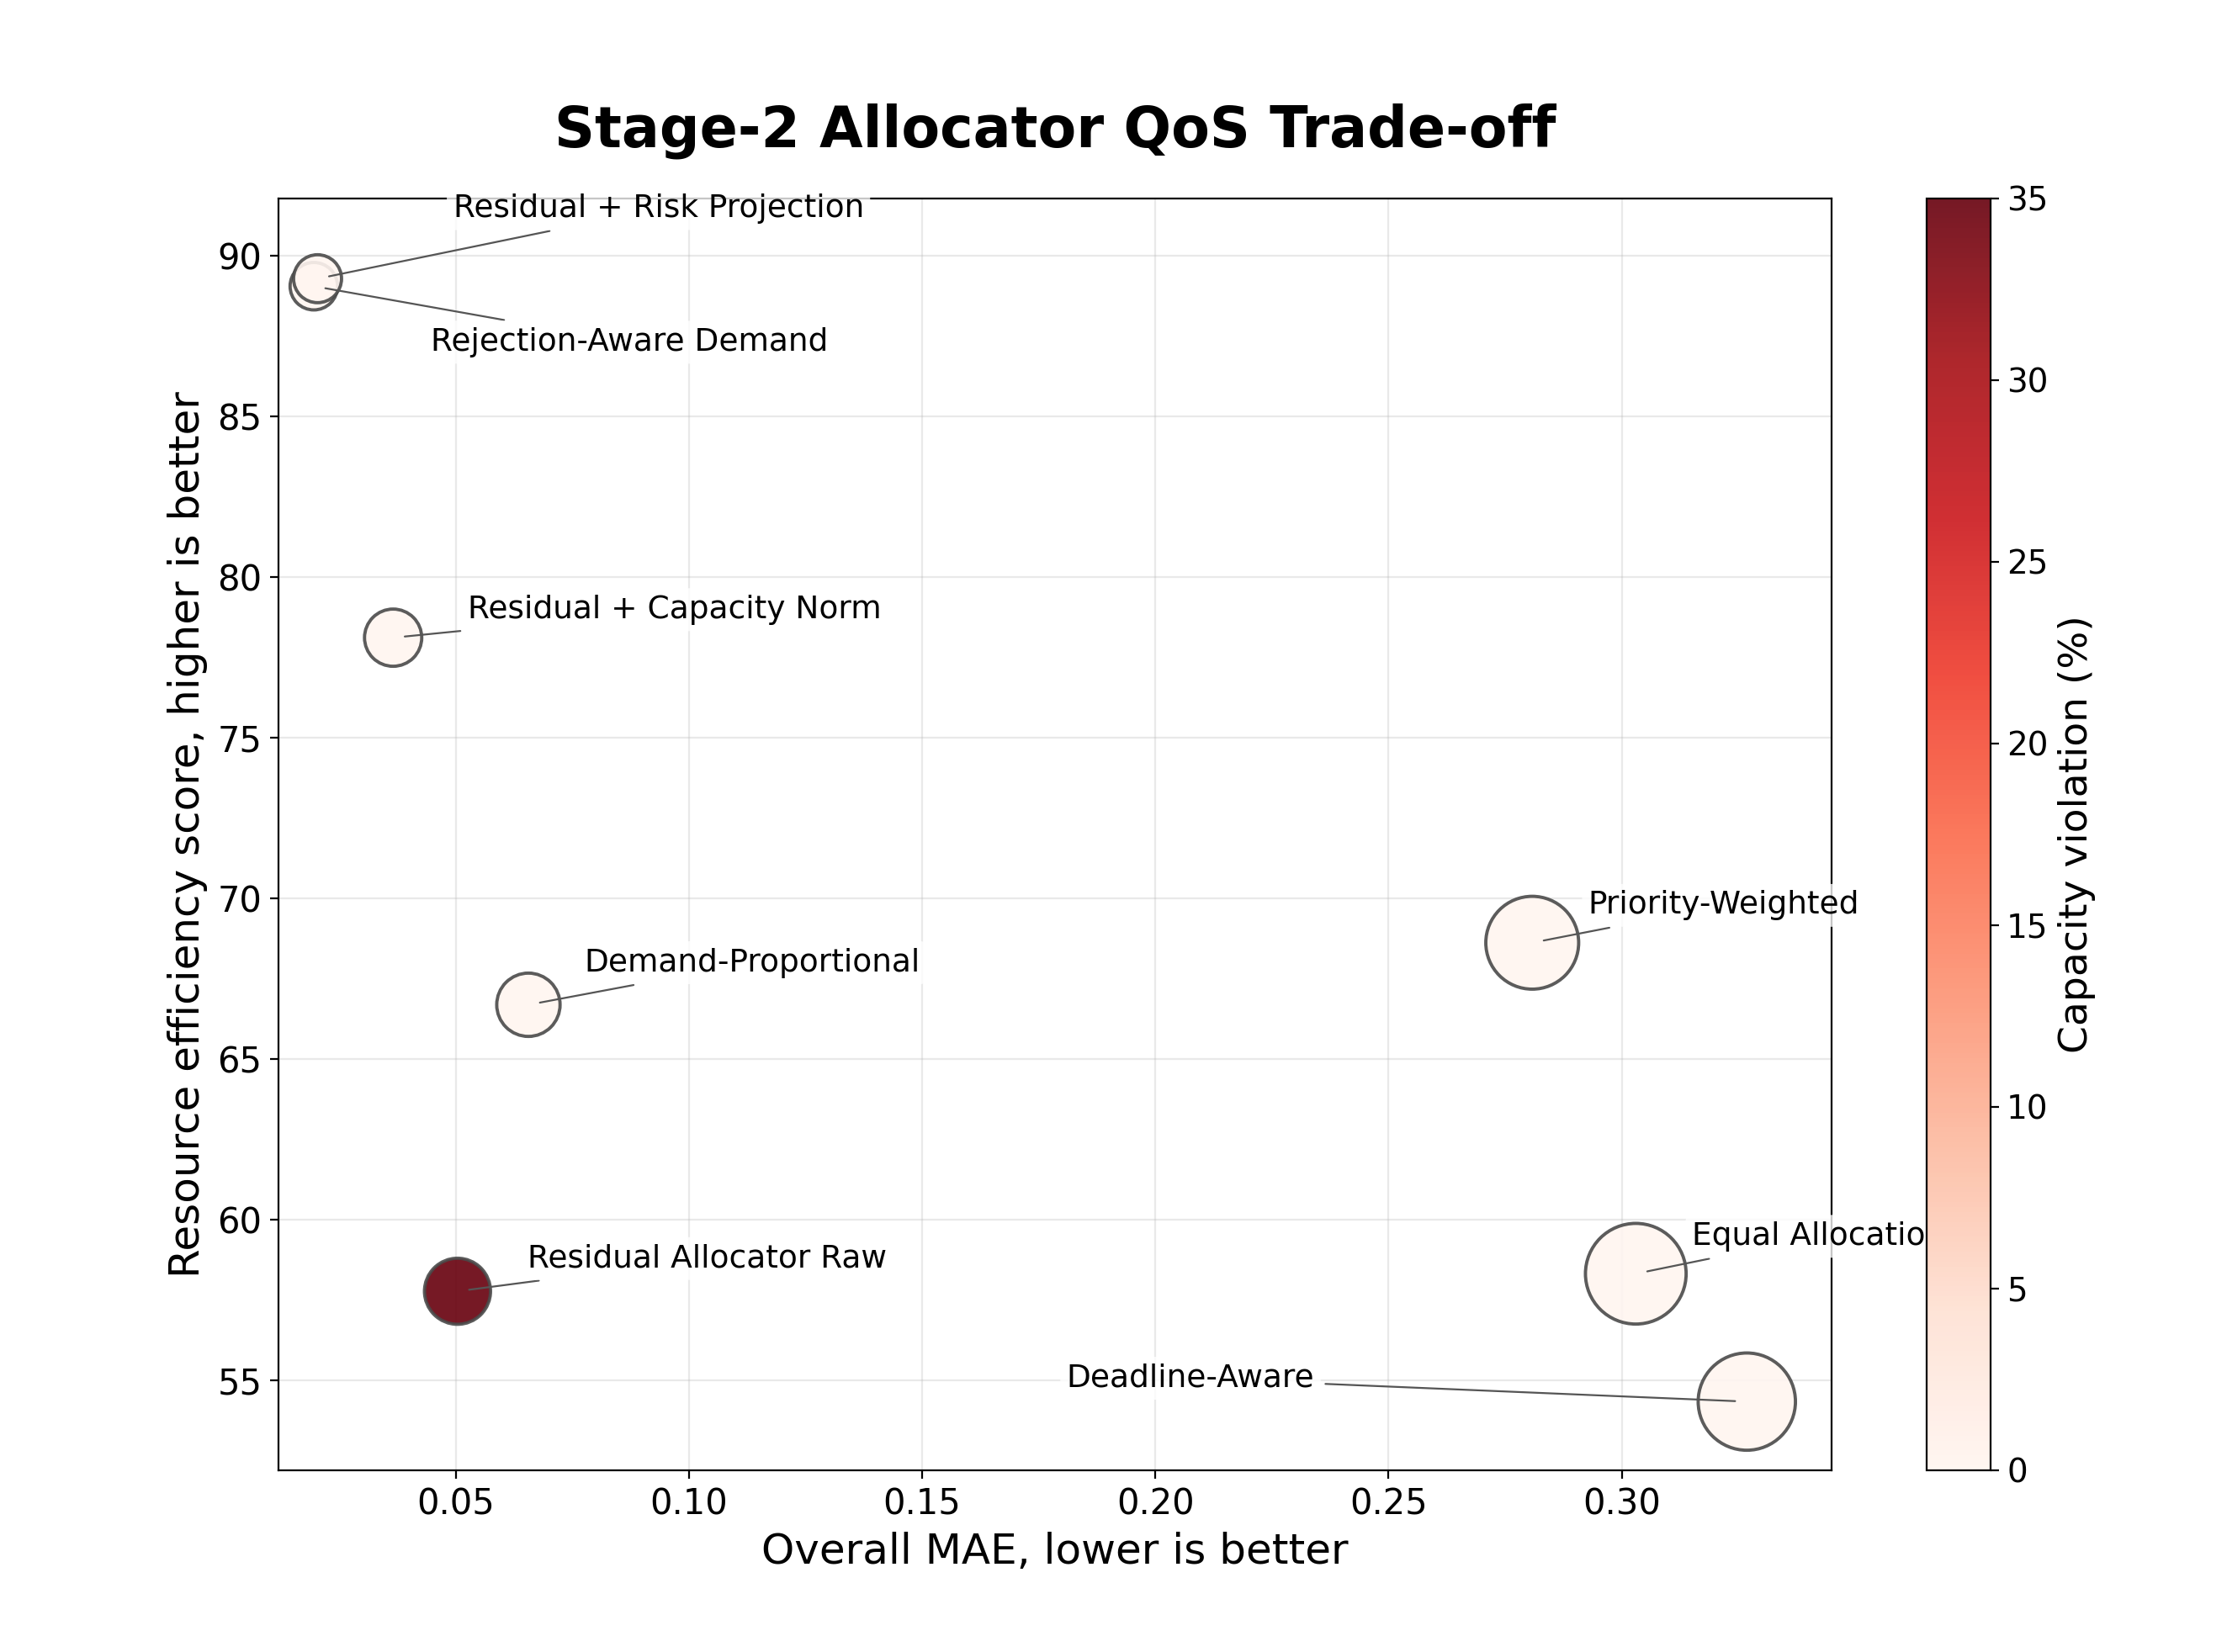
\includegraphics[width=0.80\columnwidth]{figures/results/157_fig_a8_allocator_qos_tradeoff.png}
\caption{Allocator tradeoff between resource error, under-allocation, waste, SLA risk, and efficiency.}
\label{fig:allocator_tradeoff}
\end{figure}

\begin{figure}[H]
\centering
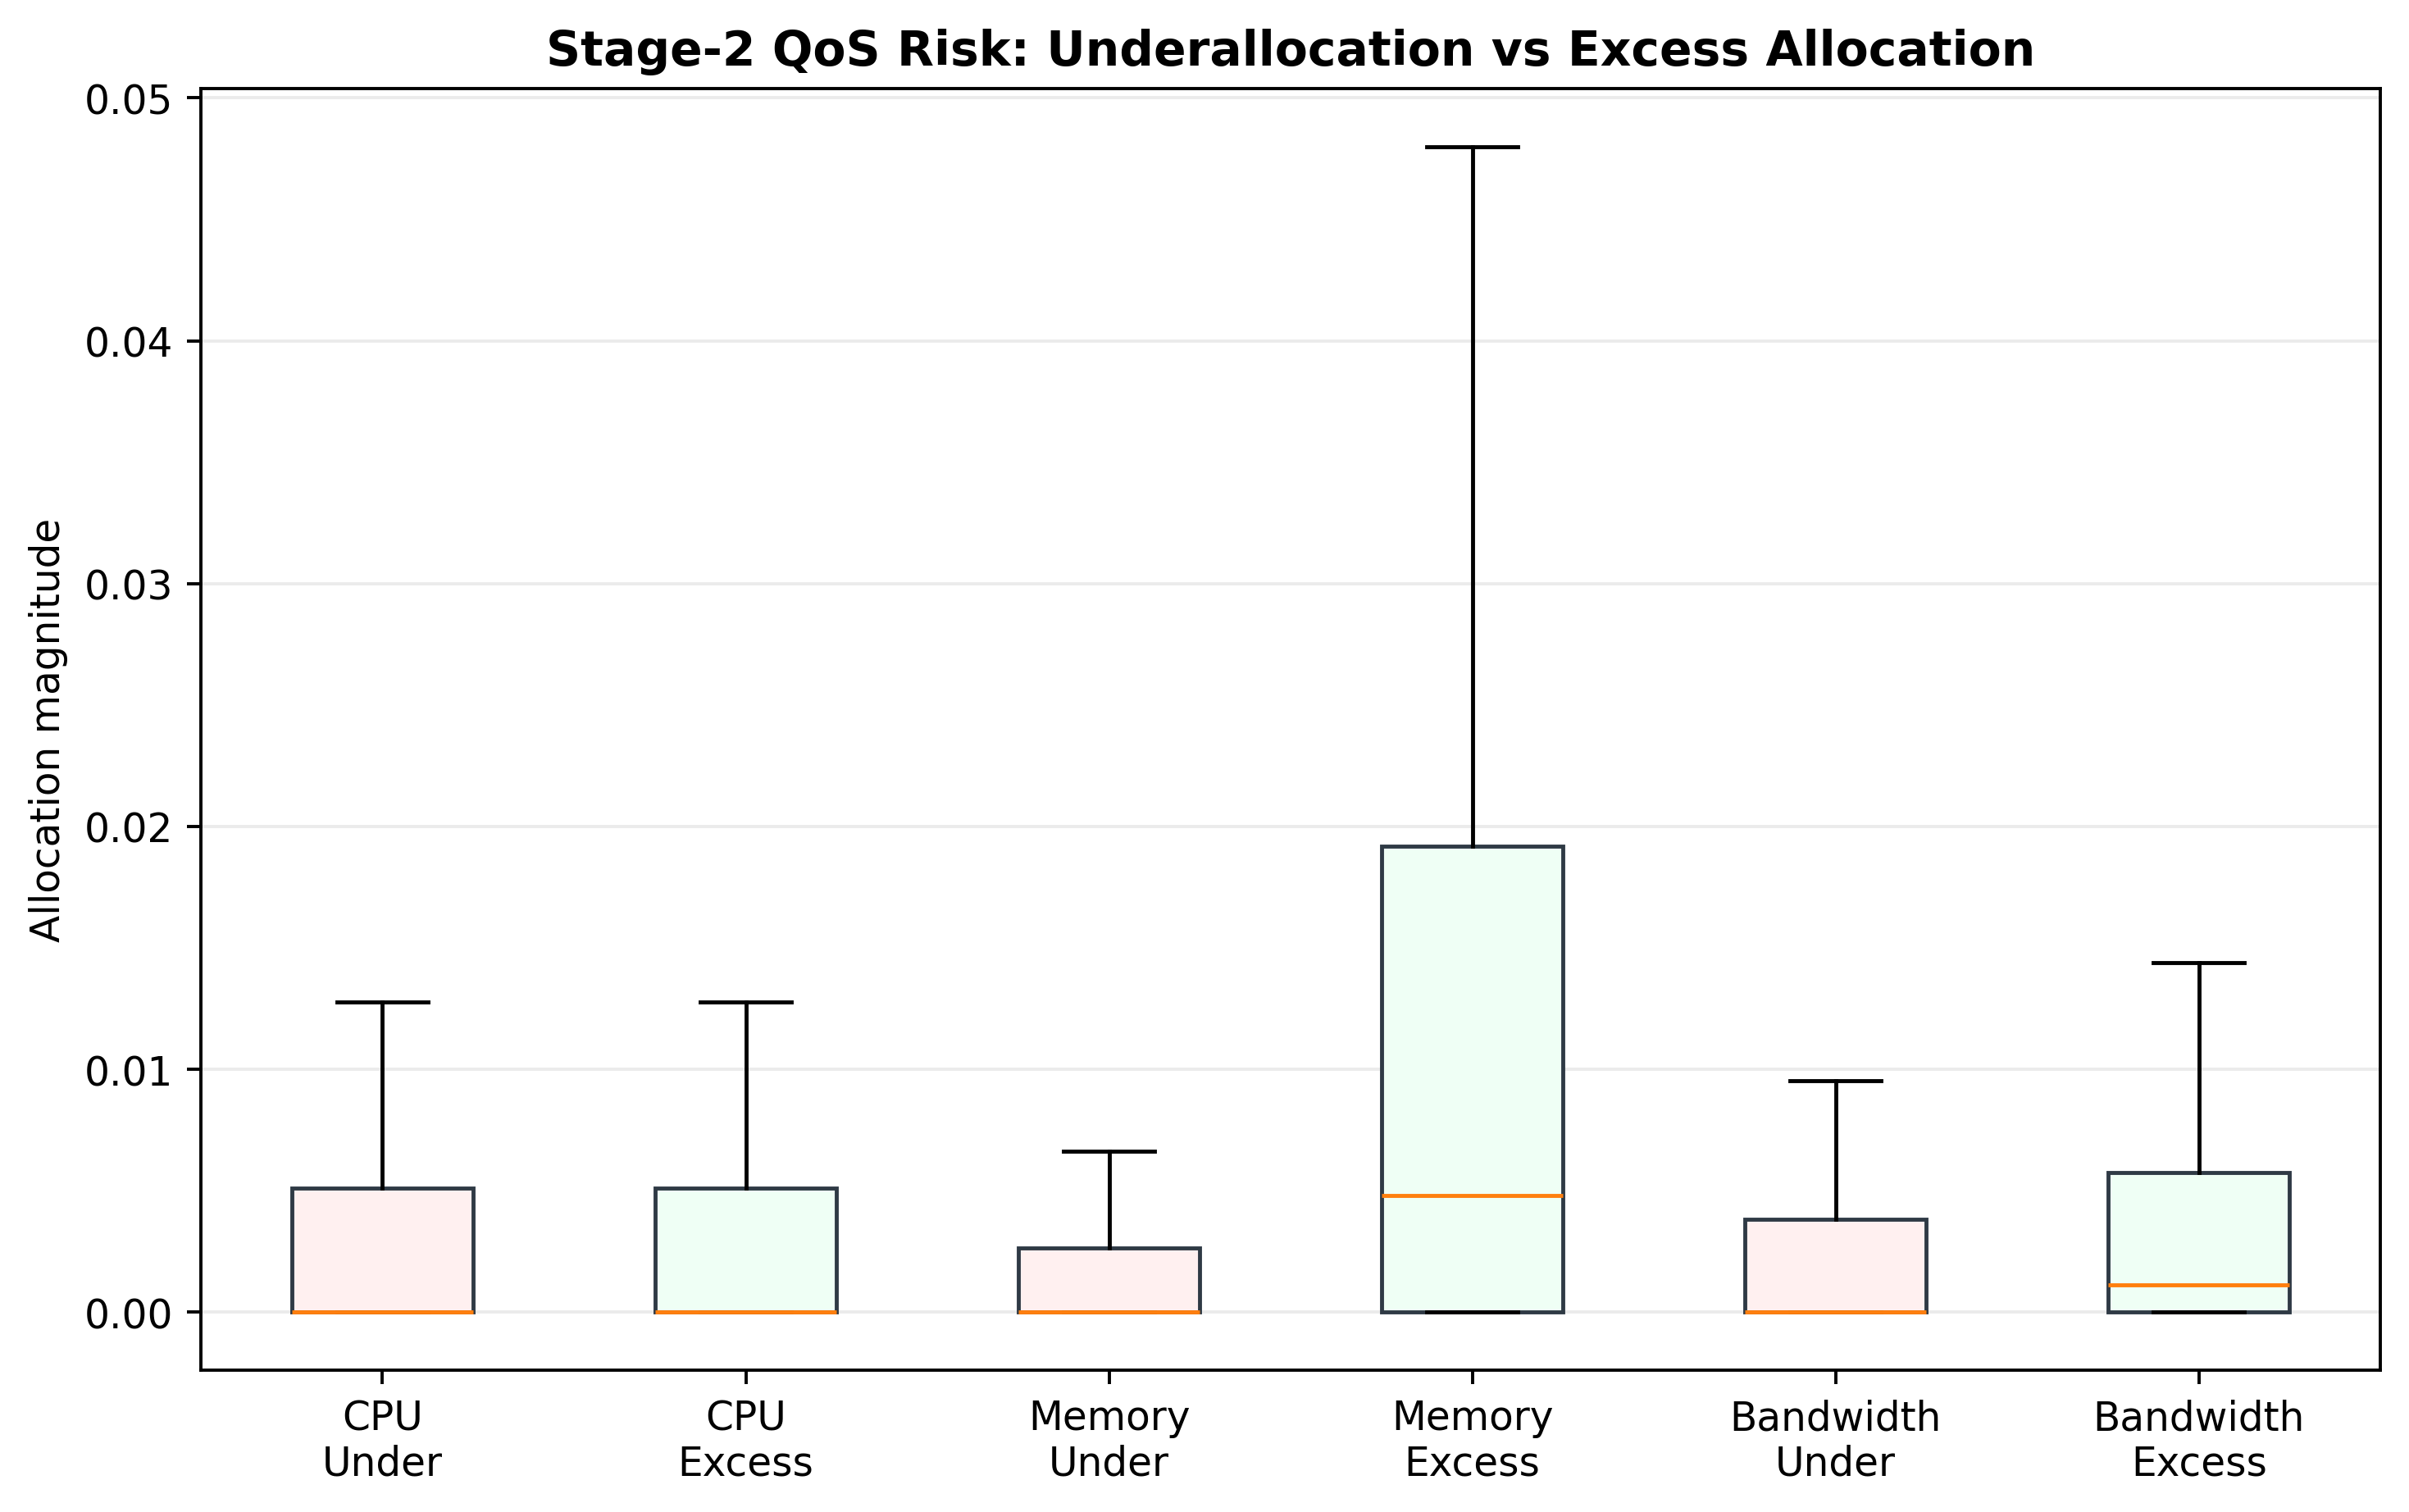
\includegraphics[width=0.80\columnwidth]{figures/diagnostics/168_fig_a21_allocator_under_vs_excess_profile.png}
\caption{Allocator under-allocation and excess profile. Capacity normalization prevents infeasible raw residual outputs from becoming final assignments.}
\label{fig:allocator_profile}
\end{figure}

\begin{figure}[H]
\centering
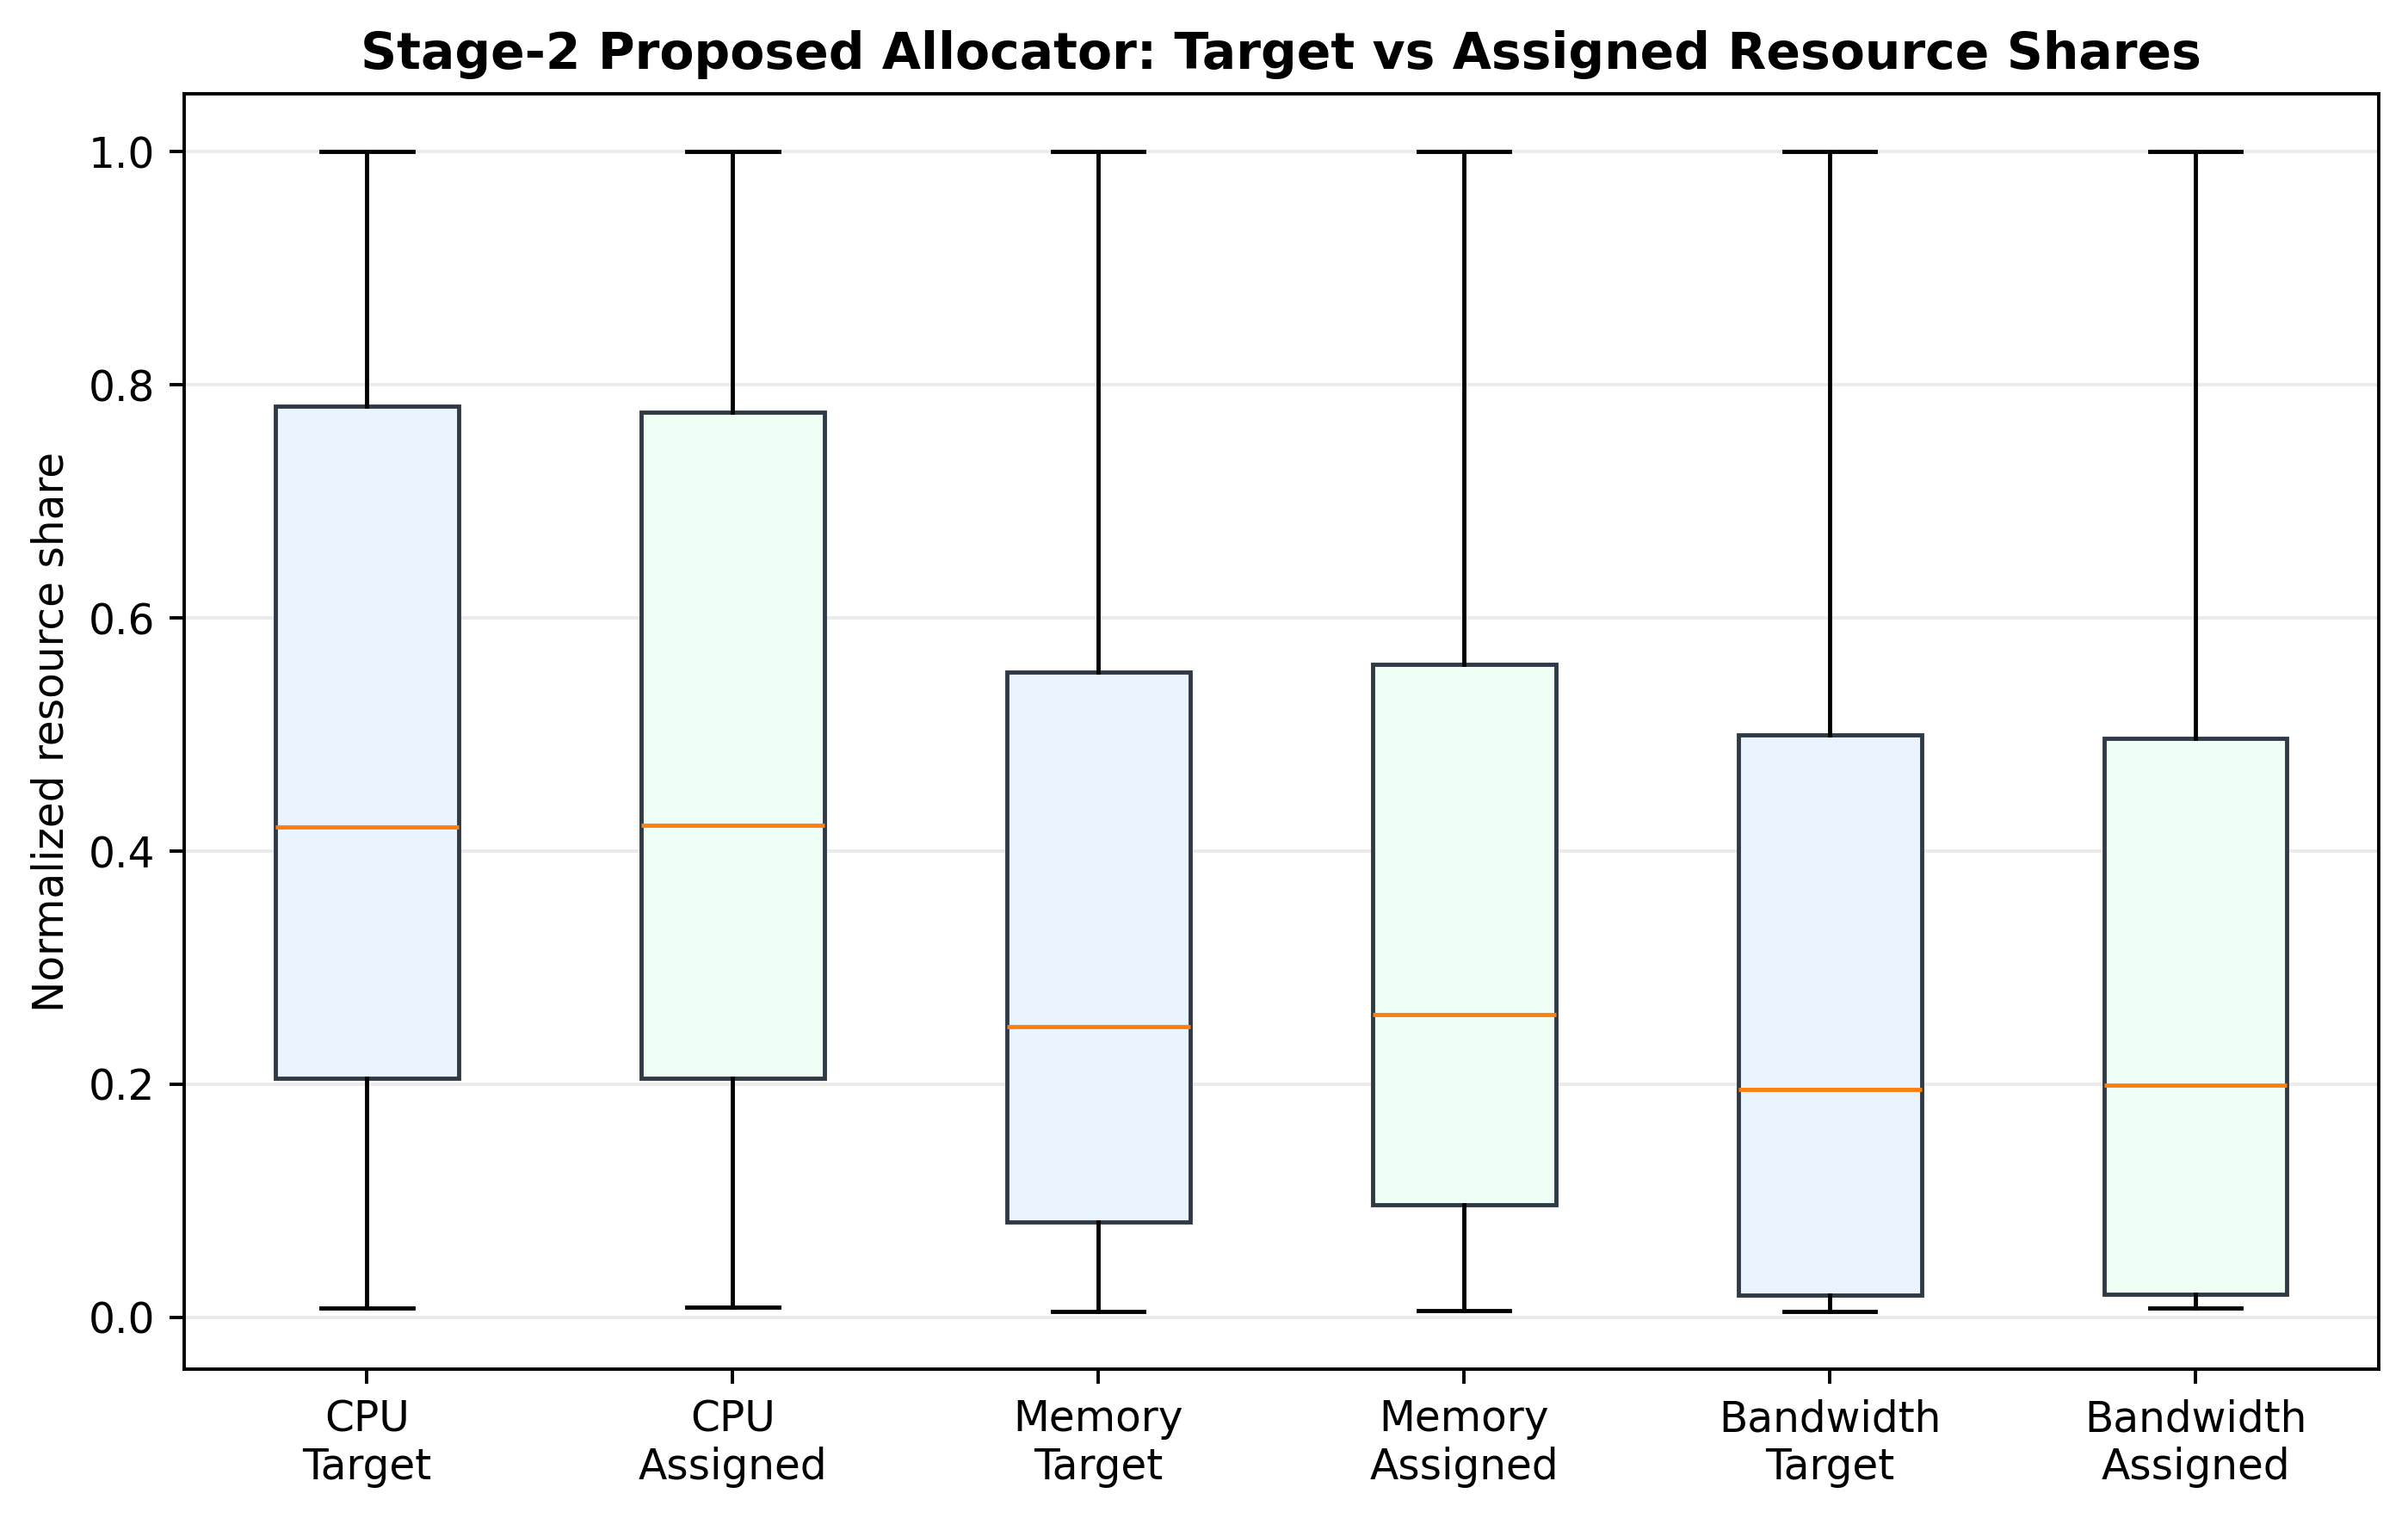
\includegraphics[width=0.84\columnwidth]{figures/diagnostics/158_fig_a9_allocator_target_vs_assigned_distribution.png}
\caption{Distribution of allocator targets and assigned resources for Stage-2 evaluation.}
\label{fig:allocator_target_distribution}
\end{figure}

\begin{figure}[H]
\centering
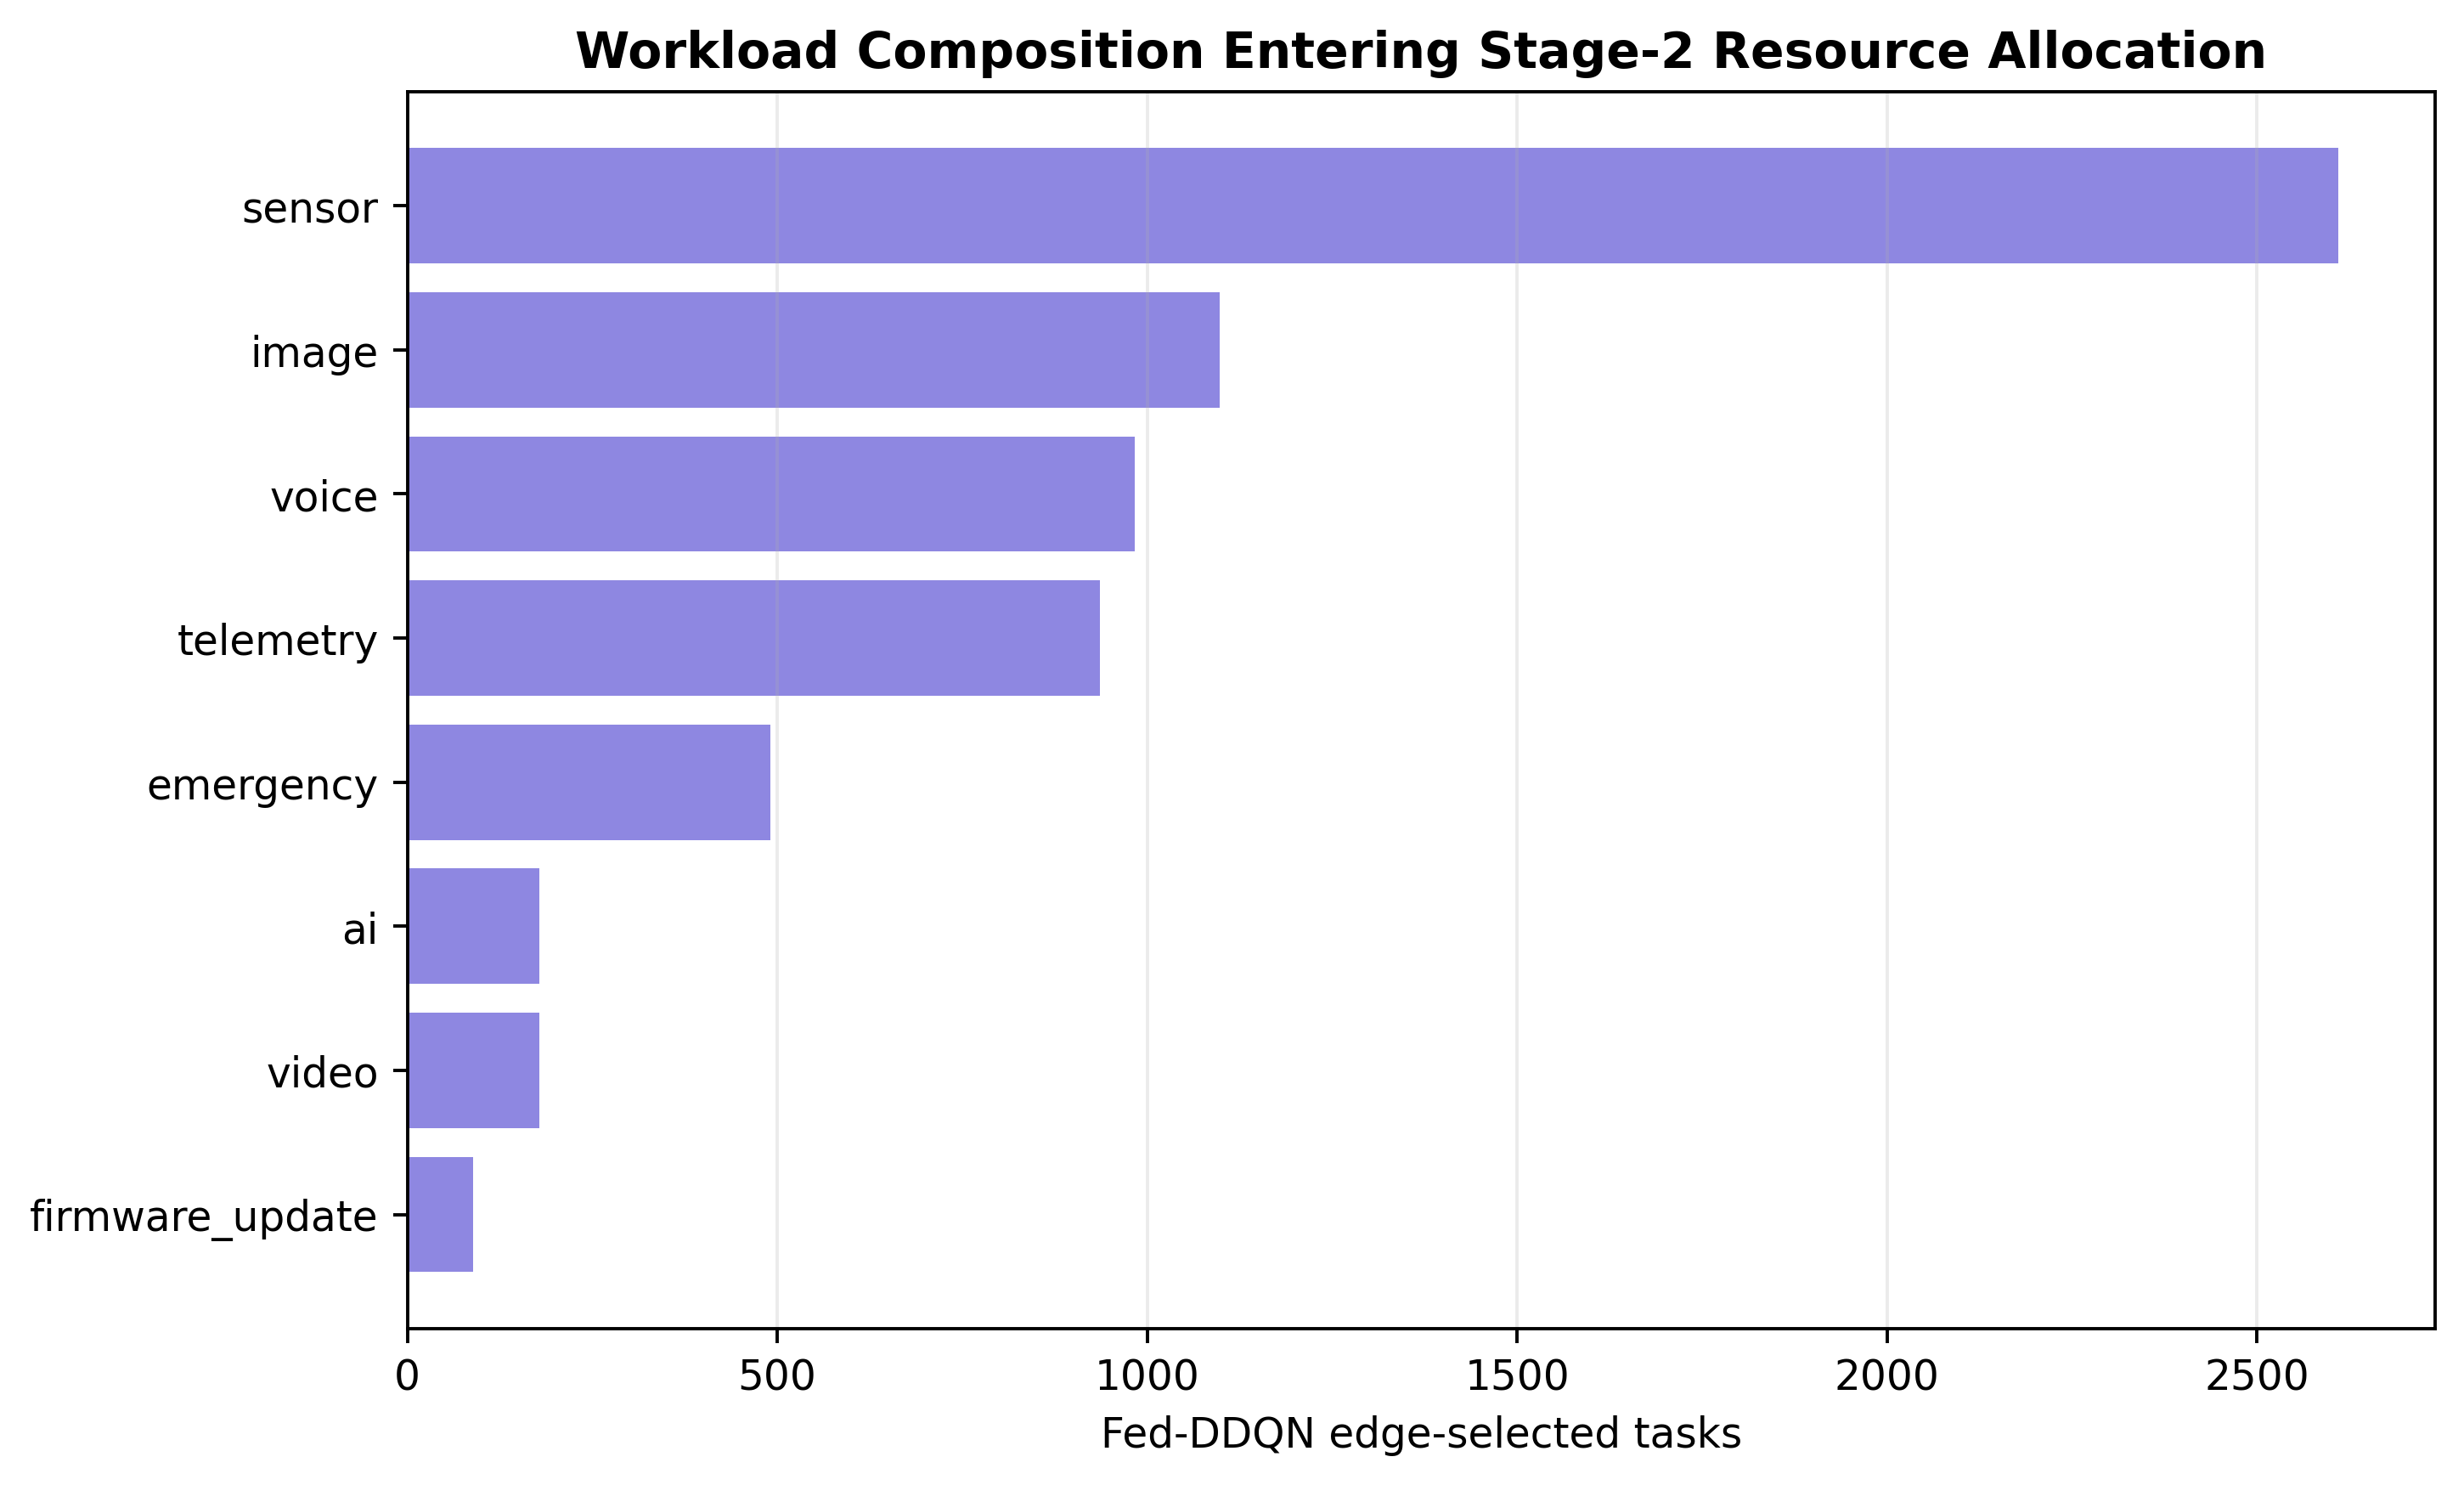
\includegraphics[width=0.84\columnwidth]{figures/diagnostics/159_fig_a10_stage2_edge_selected_task_mix.png}
\caption{Task mix among the edge-selected tasks passed to the Stage-2 allocator.}
\label{fig:stage2_task_mix}
\end{figure}

\begin{table}[H]
\centering
\caption{Task-type SLA thresholds used for QoS evaluation.}
\label{tab:sla_thresholds}
\footnotesize
\begin{tabular}{@{}lr@{}}
\toprule
Task type & SLA threshold (ms) \\
\midrule
Emergency & 50 \\
Voice & 150 \\
Sensor & 500 \\
Telemetry & 800 \\
Image & 1500 \\
Video & 3000 \\
AI & 5000 \\
Firmware update & 60000 \\
\bottomrule
\end{tabular}
\end{table}


The SLA thresholds in Table~\ref{tab:sla_thresholds} explain why the allocator
evaluation reports both average resource error and QoS-oriented measures.
Emergency and voice tasks are sensitive to short delays, whereas firmware,
video, and AI workloads tolerate longer execution windows but can consume more
capacity. This task-dependent tolerance is the reason the Stage-2 results are
reported with under-allocation, waste, SLA-risk, and efficiency metrics instead
of a single aggregate error value.

The ablation plot in Fig.~\ref{fig:allocator_ablation_efficiency} complements
the allocator tables by showing that the final residual-plus-risk-projection
variant is not only a lower-error model. It combines learned correction with
capacity-safe projection, keeping the final allocator assignment feasible while
reducing high-risk under-allocation cases.

\begin{figure}[H]
\centering
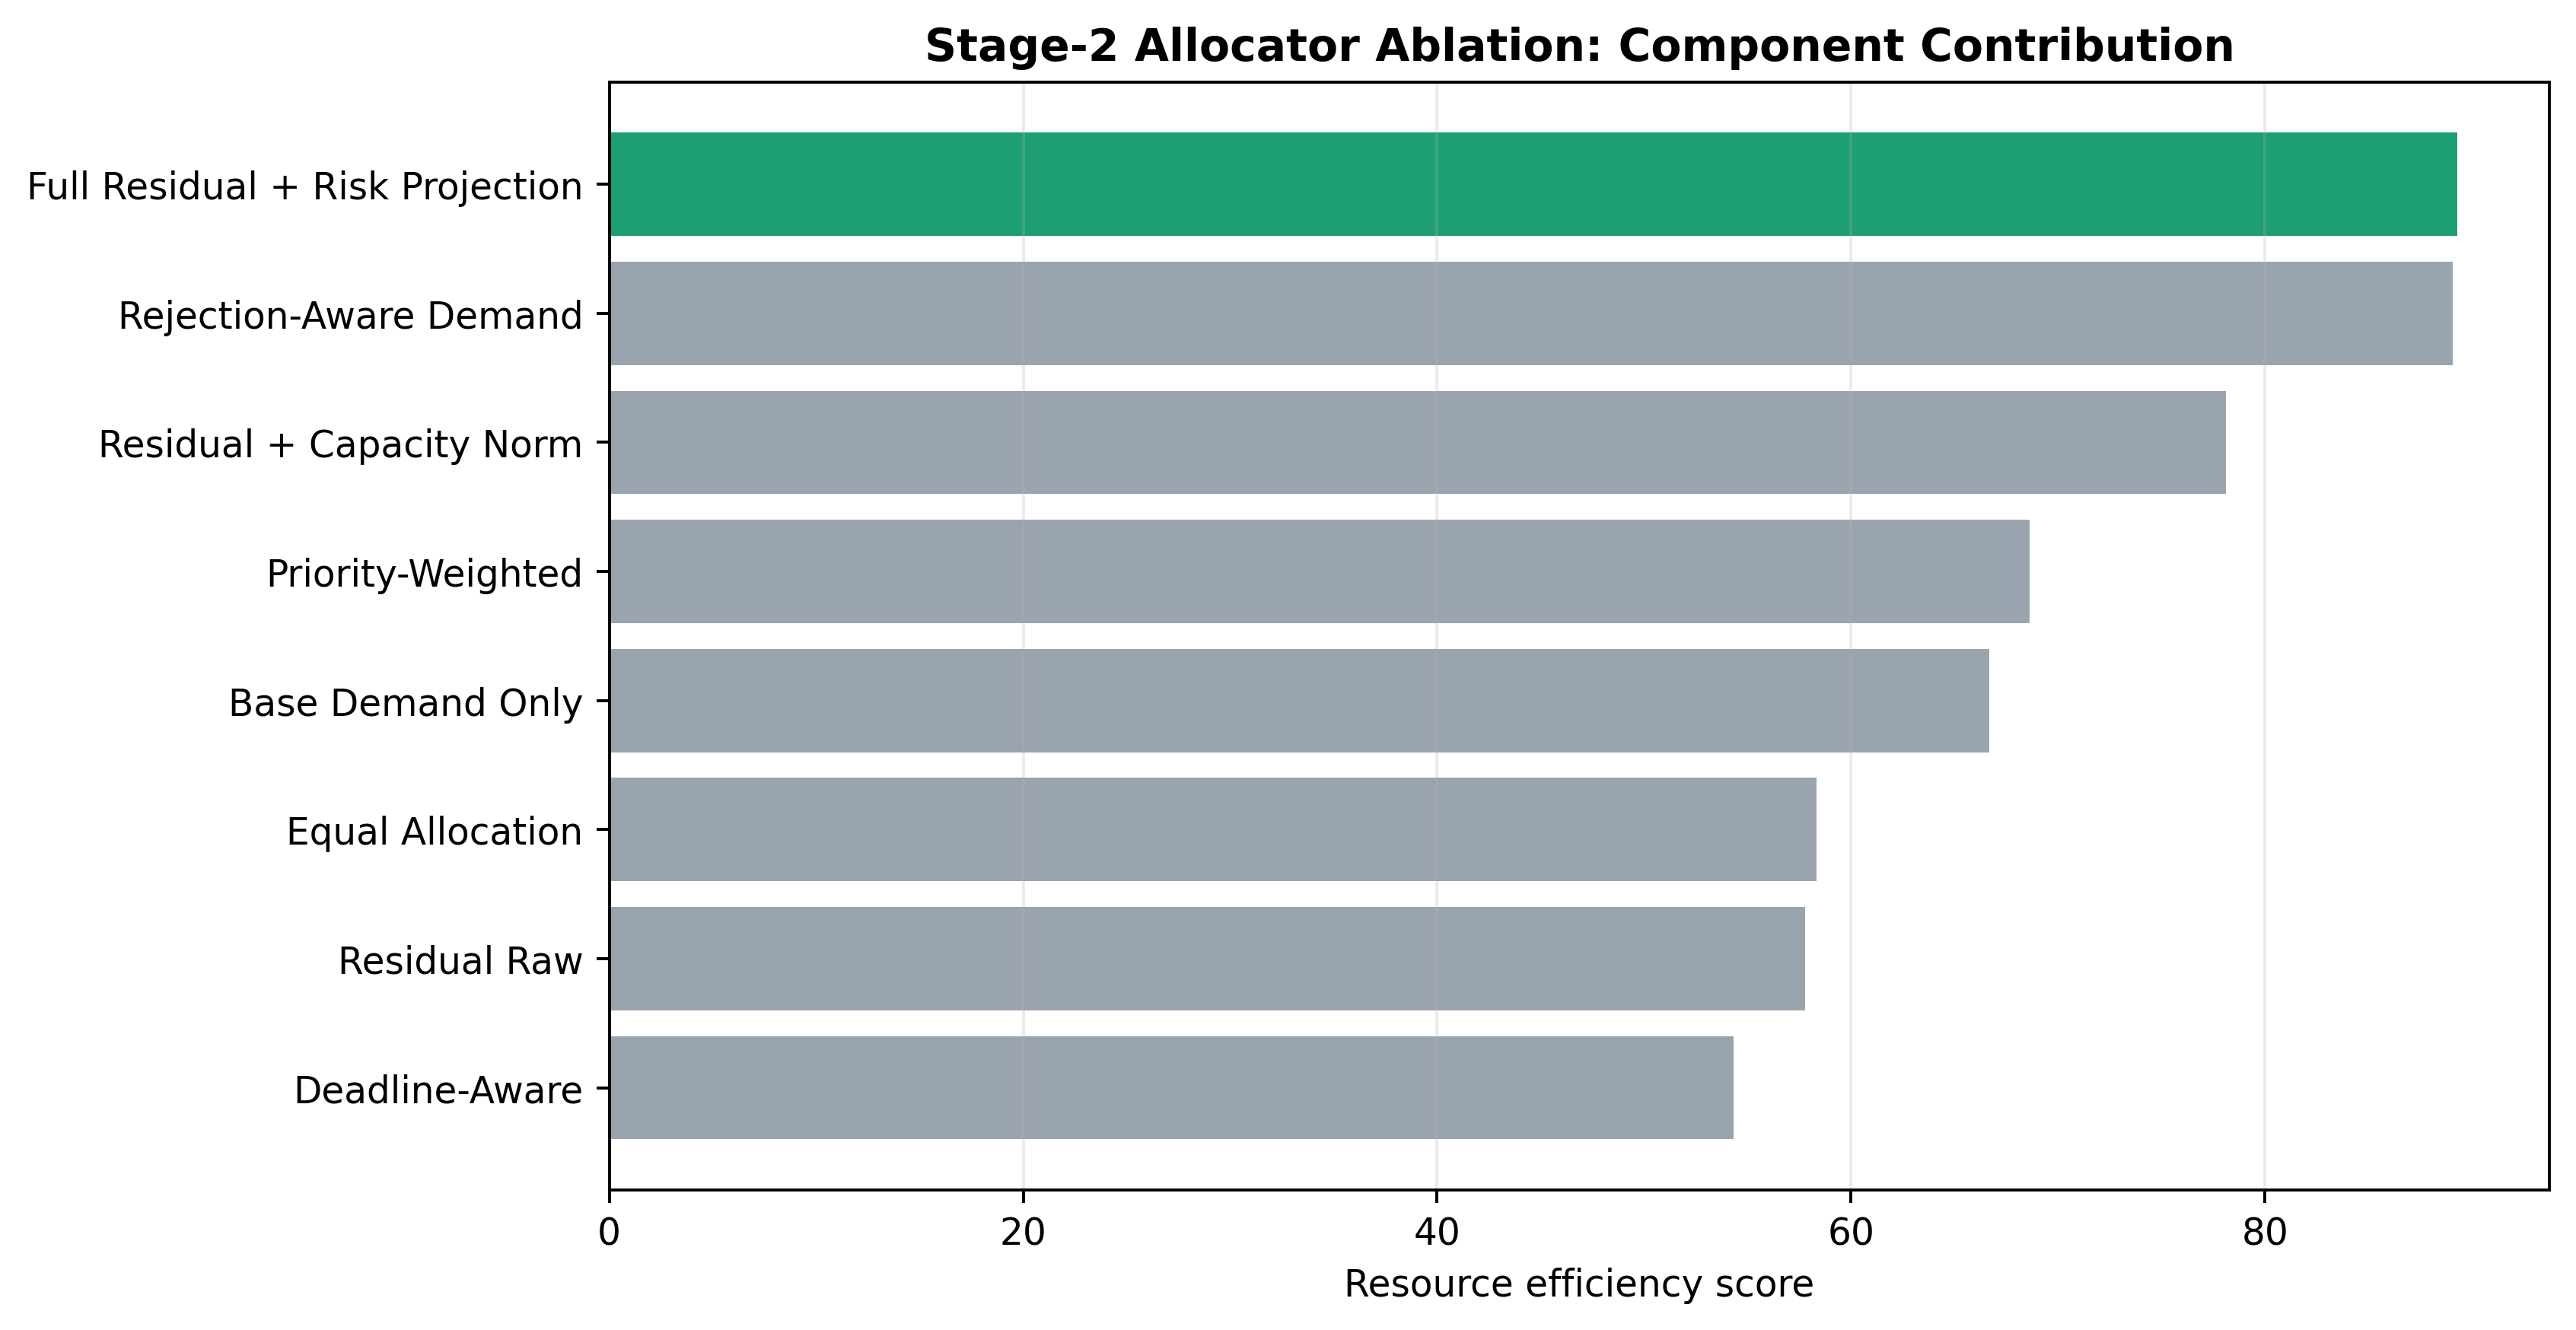
\includegraphics[width=0.84\columnwidth]{figures/diagnostics/160_fig_a11_allocator_ablation_efficiency.png}
\caption{Allocator ablation efficiency comparison.}
\label{fig:allocator_ablation_efficiency}
\end{figure}

\FloatBarrier
